%  TEX program=xelatex

\documentclass[12p,UTF8]{article}
\setlength\paperheight{26cm}
\setlength\paperwidth{18.4cm}
\usepackage[fontset=windows,zihao={-4}]{ctex} % Chinese support, using Windows fonts
\usepackage{setspace} % 导入 setspace 宏包
\usepackage{graphicx} % Insert images
\usepackage{listings} % Print source code
\usepackage{color} % Color support
\usepackage{booktabs} % Professional table support
\usepackage{pdflscape} % Landscape pages support in PDF
\usepackage{hyperref} % Hypertext links support for cross-referencing
\usepackage{geometry} % Page layout customization
\usepackage{float}
\usepackage{subfigure}
\usepackage{amsmath}
\usepackage{placeins}
% 
% \geometry{left = 8 cm, right=8cm , top = 3cm, bottom = 3cm}
% Customize hyperref format (it's set to no special format here)
\hypersetup{hidelinks}
\setstretch{1.25}
% 设置全局页面边距
\geometry{left=3.17cm, right=3.17cm, top=2.54cm, bottom=2.54cm}
% Declare directories to search for graphics files for graphicx
\graphicspath{{figures/}{logo/}}



% Define new command for title page
\newcommand{\reporttitle}[2]{
  \LARGE\textsf{#1}\quad\underline{\makebox[12em]{#2}}
}
\newcommand{\reportinfo}[2]{
  \large\makebox[4em]{\textsf{#1}}\quad\underline{\makebox[15em]{#2}}
}

% The document begins here
\begin{document}
\begin{spacing}{1.25} % 设置全局行距为1.25倍
  \begin{titlepage}
     \centering
     % \vspace*{0.2\fill}
     % \vspace*{-20pt}
     \includegraphics[width=\linewidth]{ahu1.bmp}\\[3cm] % Change the school logo here (See the logo/ directory) and adjust the height
     % \includegraphics[height=144pt]{pku-text-logo}\\[48pt] % Change the school logo here (See the logo/ directory) and adjust the height
     % {\huge\textsf{课\ 程\ 实\ 验\ 报\ 告}}\\[48pt]
     {\zihao{2} \heiti《电子线路》\ 综\ 合\ 作\ 业}\\[4cm]
     % \reporttitle{实验名称}{立扫帚实验}\\[72pt]
     % \reportinfo{课程名称}{麻瓜研究}\\[8pt]
     \reportinfo{\zihao{-2}\songti 学\hspace{\fill}院}{\zihao{-2}\songti 电子信息工程学院}\\[10pt]
     \reportinfo{\zihao{-2}\songti 专\hspace{\fill}业}{\zihao{-2}\songti 通信工程专业}\\[8pt]
     \reportinfo{\zihao{-2}\songti 年\hspace{\fill}级}{\zihao{-2} \songti 23级}\\[8pt]
     \reportinfo{\zihao{-2}\songti 学\hspace{\fill}号}{\zihao{-2}\songti P22314040}\\[8pt]
     \reportinfo{\zihao{-2}\songti 姓\hspace{\fill}名}{\zihao{-2}\songti 汪攀}\\
     \vspace*{\fill}
  \end{titlepage}
  % \newgeometry{left = 3.17cm, right = 3.17cm, top = 2.54cm , bottom=2.54cm}
  \tableofcontents
  \newpage
 \songti

  \section{题目描述}
共源放大器指标仿真测量,参考电路如下,该管VGS(th)=1.72V要求:
\\  (1)直流静态工作点MOS管栅极、源极和漏极电压;
\\  (2)负载为10kΩ时的电压和电流增益增益;
\\  (3)输入电阻测量,给出测量时的仿真电路图及结果;
\\  (4)输出电阻测量,给出测量时仿真电路图及结果。

\begin{figure}[h]
  \centering
  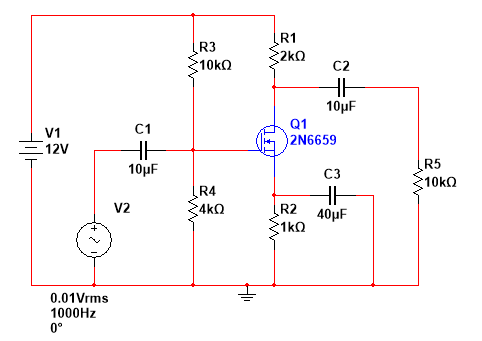
\includegraphics[width=1\linewidth]{timu.png}
  \caption{共源放大器电路图}
  \label{fig:circuit}
\end{figure}

\section{设计过程}

\subsection{直流静态工作点测量}
首先将电路进行搭建。根据题目要求,我们需要测量MOS管的直流静态工作点,即栅极、源极和漏极的电压。为此,我们需要在电路中添加一个直流电源后来测量这些电压。
测得:
\begin{itemize}
  \item 栅极电压$V_g=3.43V$
  \item 漏极电压$V_d=8.83.V$
  \item 源极电压$V_s=1.59V$。
\end{itemize}
所以$V_{gs}=V_g-V_s=1.84V$>$V_{gs(th)}=1.72V$,\\
$V_{ds}=V_d-V_s=7.24V>V_{gs}-V_{gs(th)}=0.12V$,满足要求,mos管工作在放大状态。
\begin{figure}[h]
  \centering
  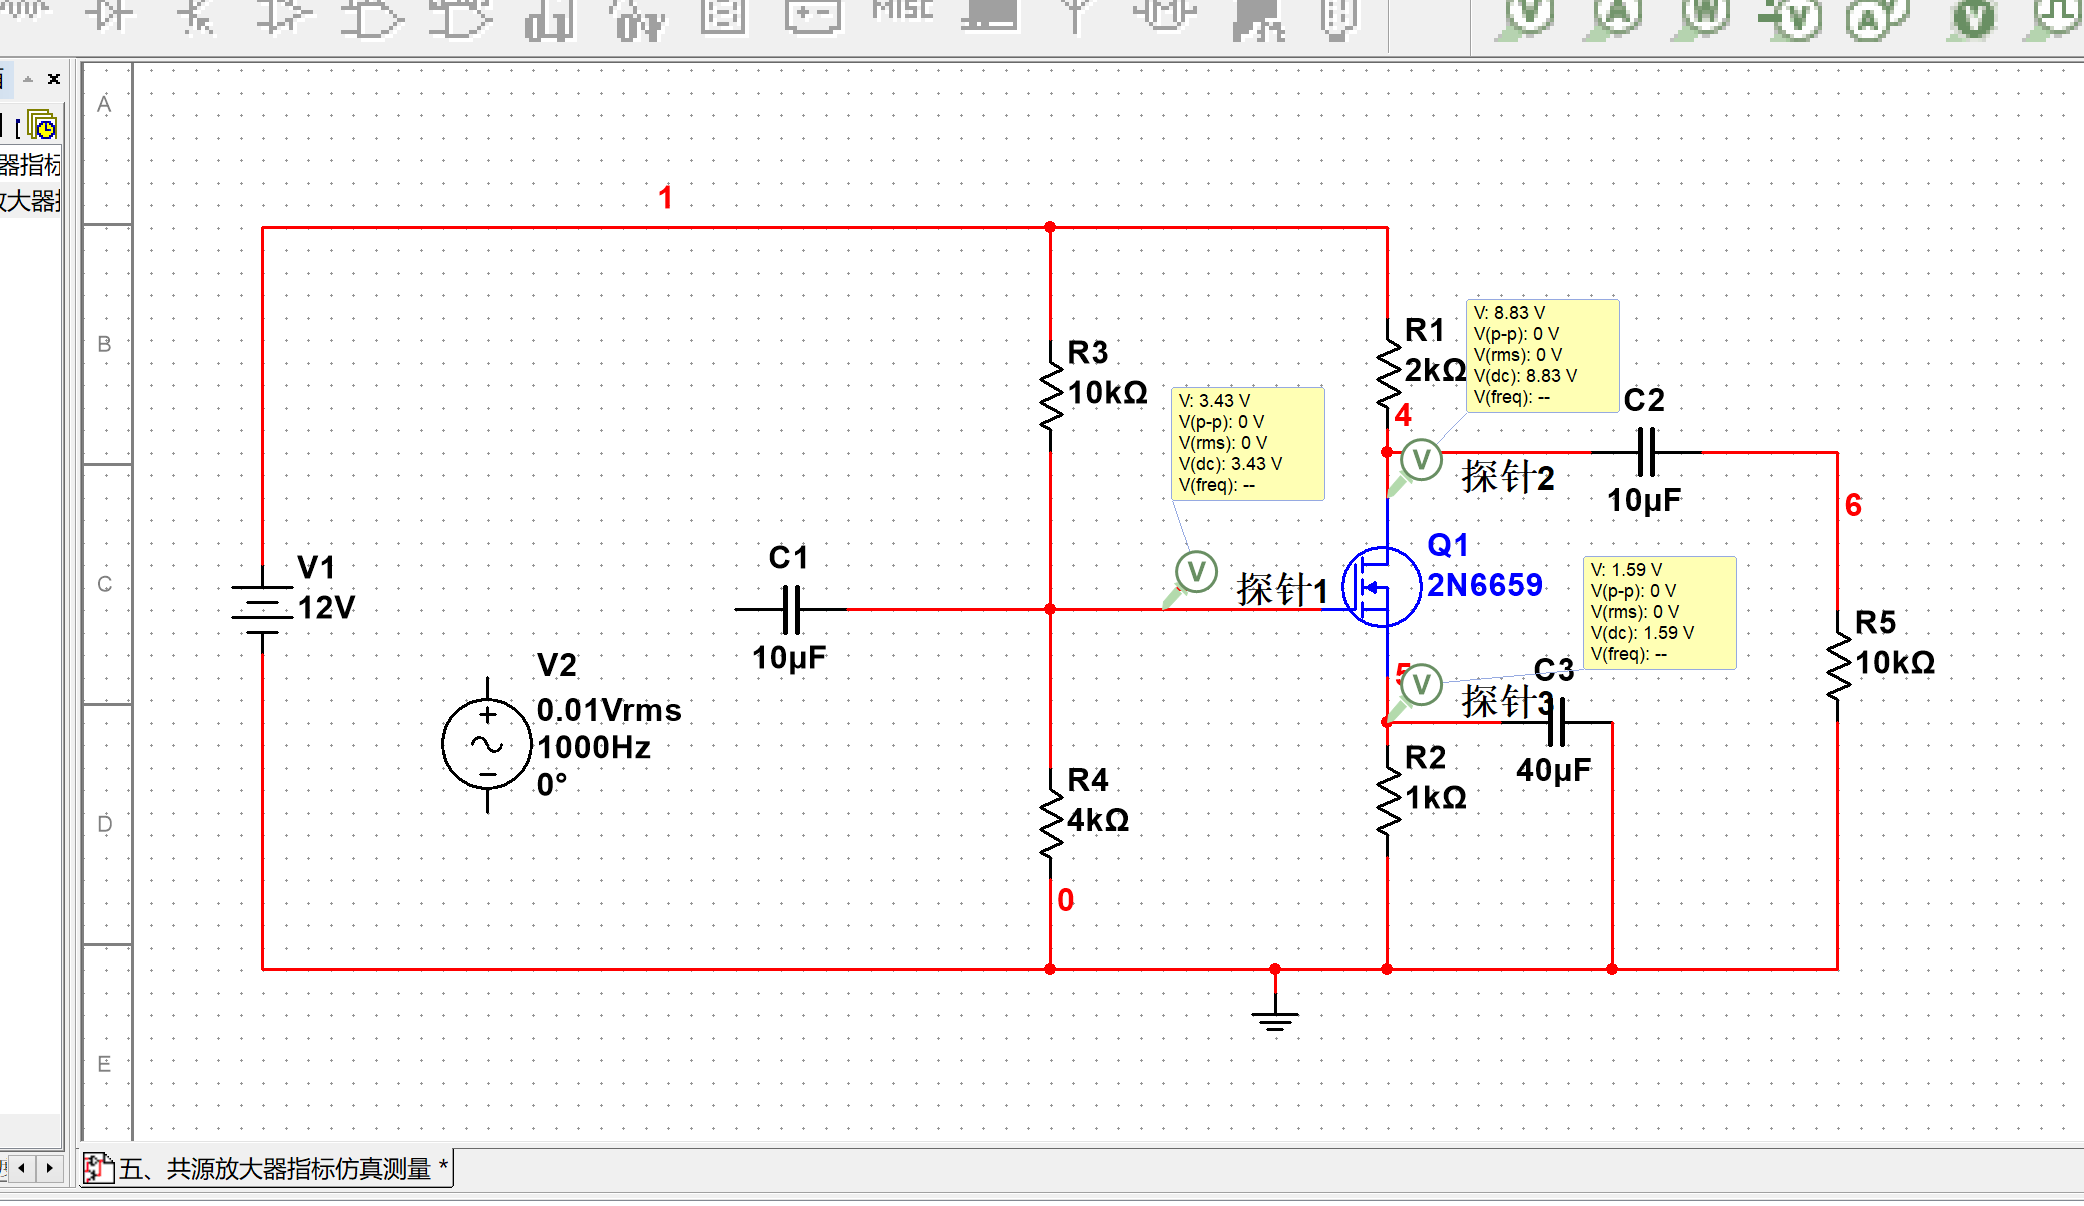
\includegraphics[width=1\linewidth]{1.png}
  \caption{直流静态工作点测量}
  \label{fig:circuit}
\end{figure}

\subsection{负载为10kΩ时的电压和电流增益增益测量}
在测量中:
\begin{itemize}
  \item 输入信号有效值$V_{in} =0.01 {V}$
  \item 输入信号的频率$f=1\text{kHz}$
  \item 负载电阻$R_L = 10\ \text{k}\Omega$
\end{itemize}

通过仿真得到:
\begin{align*}
  V_{in}  &=10\ \text{mV} \\
  V_{out} &= 447.633\ \text{mV} \\
  I_{in}  &= 57.44\ \text{nA} \approx 0 \\
  I_{out} &= 44.763\ \text{uA} \\
  A_v &= \frac{V_{out}}{V_{in}} = \frac{447.635}{10} \approx 44.8 
\end{align*}
所以共源放大器没有电流增益,电压增益为44.8
\begin{figure}[H]
  \centering
  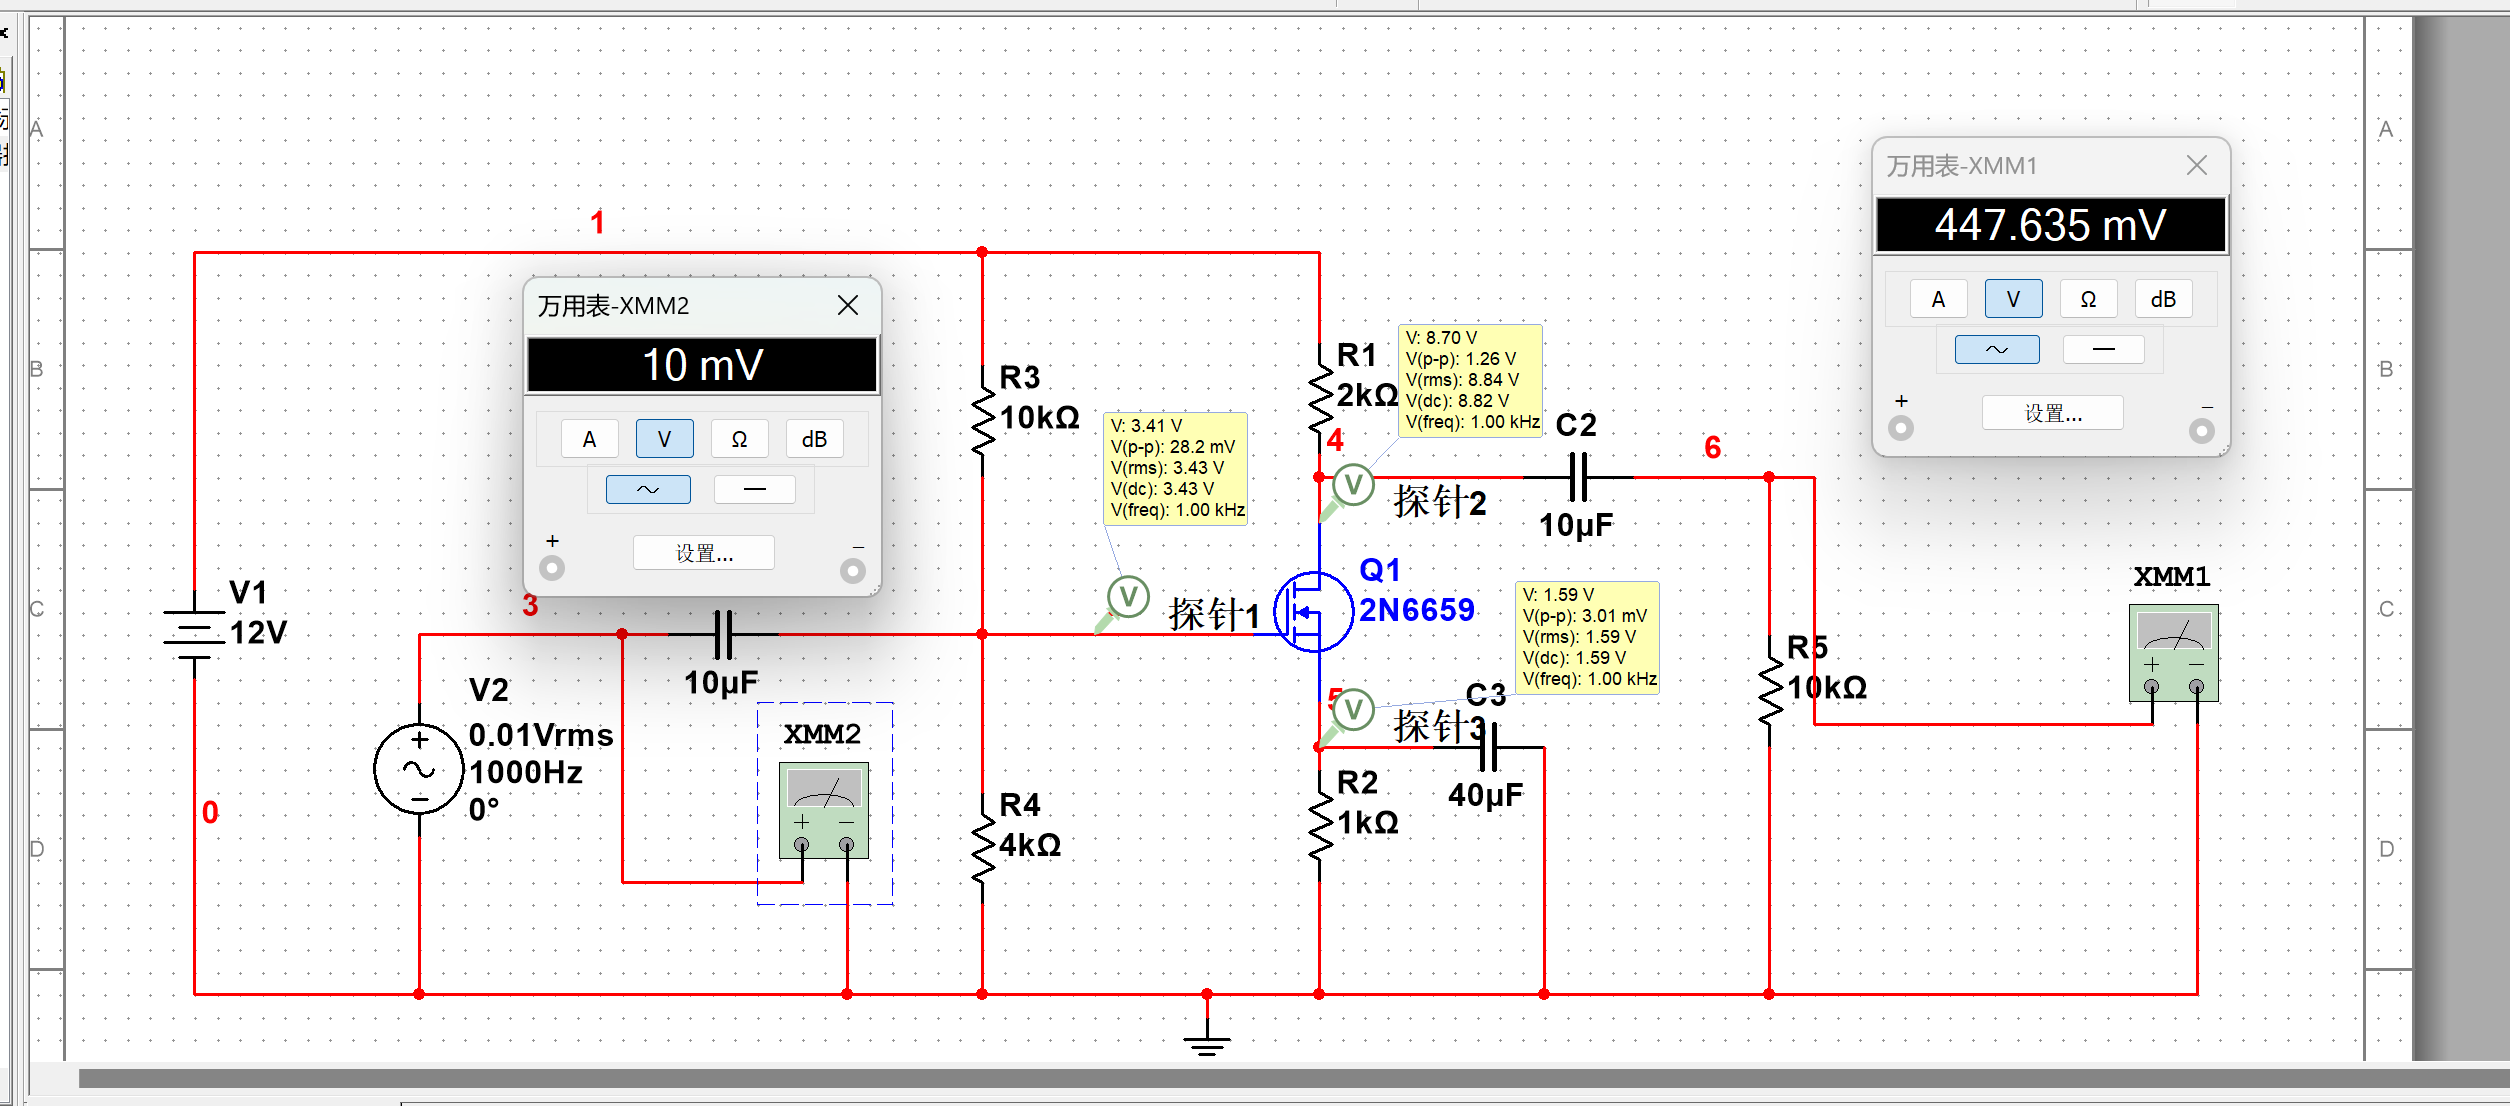
\includegraphics[width=1\linewidth]{2.png}
  \caption{负载为10kΩ时的电压增益测量}
  \label{fig:circuit}
\end{figure}
\begin{figure}[H]
  \centering
  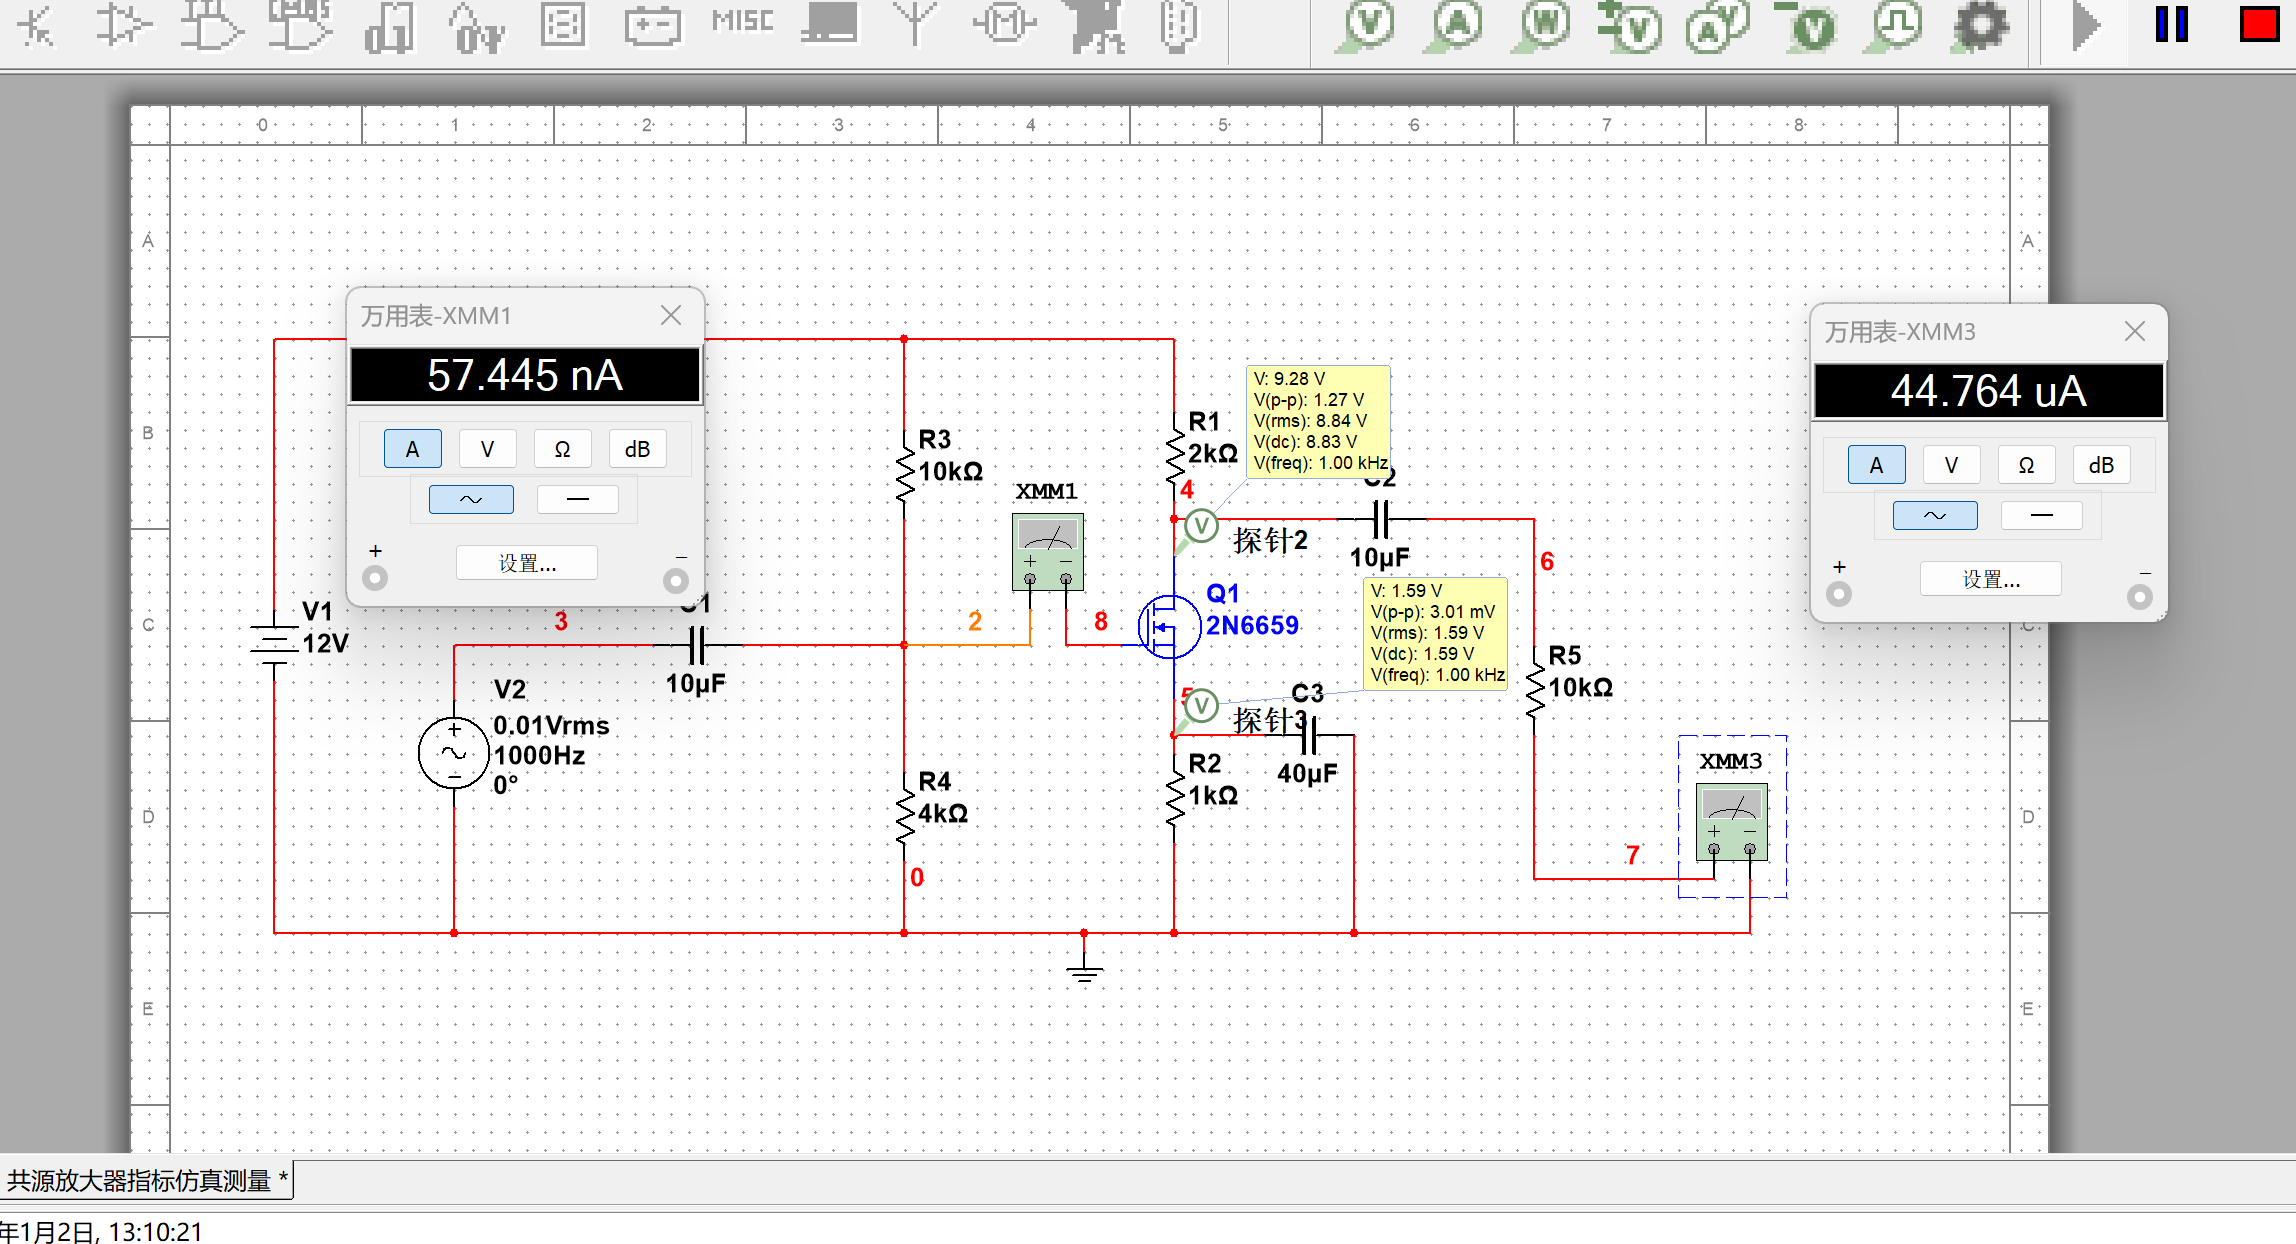
\includegraphics[width=1\linewidth]{3.png}
  \caption{负载为10kΩ时的电流增益测量}
  \label{fig:circuit}
\end{figure}

\subsection{输入电阻测量}
根据本学期模电实验的《模拟电子技术基础实验指导》为了测量输入电阻$R_{in}$,我们需要在电路输入端串联一个已知的测试电阻$R_{test}$(根据分析,当$U_s$固定,$U_i$大约为$U_s$的一半的时候测量误差最小,所以选择该测试电阻大小近似于输入电阻),并通过测量信号源输出电压$V_{s}$和输入电压$V_{in}$来计算。
首先进行理论计算:
\begin{align*}
  R_{in} &\approx R_3//R_4 \approx 2.857\ \text{k}\Omega \\
\end{align*}
\begin{itemize}
  \item 选择测试电阻$R_{test} = 2.8\ \text{k}\Omega$。
  \item 测量得到信号源输出电压$V_{s} = 10\ \text{mV}$。
  \item 测量得到输入电压$V_{in} = 5.055\ \text{mV}$。
\end{itemize}

输入电阻计算公式为:
\[
R_{in} = R_{test} \cdot \frac{V_{in}}{V_s-V_{in}}
\]

代入数据计算得:
\[
R_{in} = 2.8\ \text{k}\Omega \cdot \frac{5.055}{10-5.055}  \approx 2.86\ \text{k}\Omega
\]
仿真结果与理论计算结果一致。
\FloatBarrier
\begin{figure}[H]
  \centering
  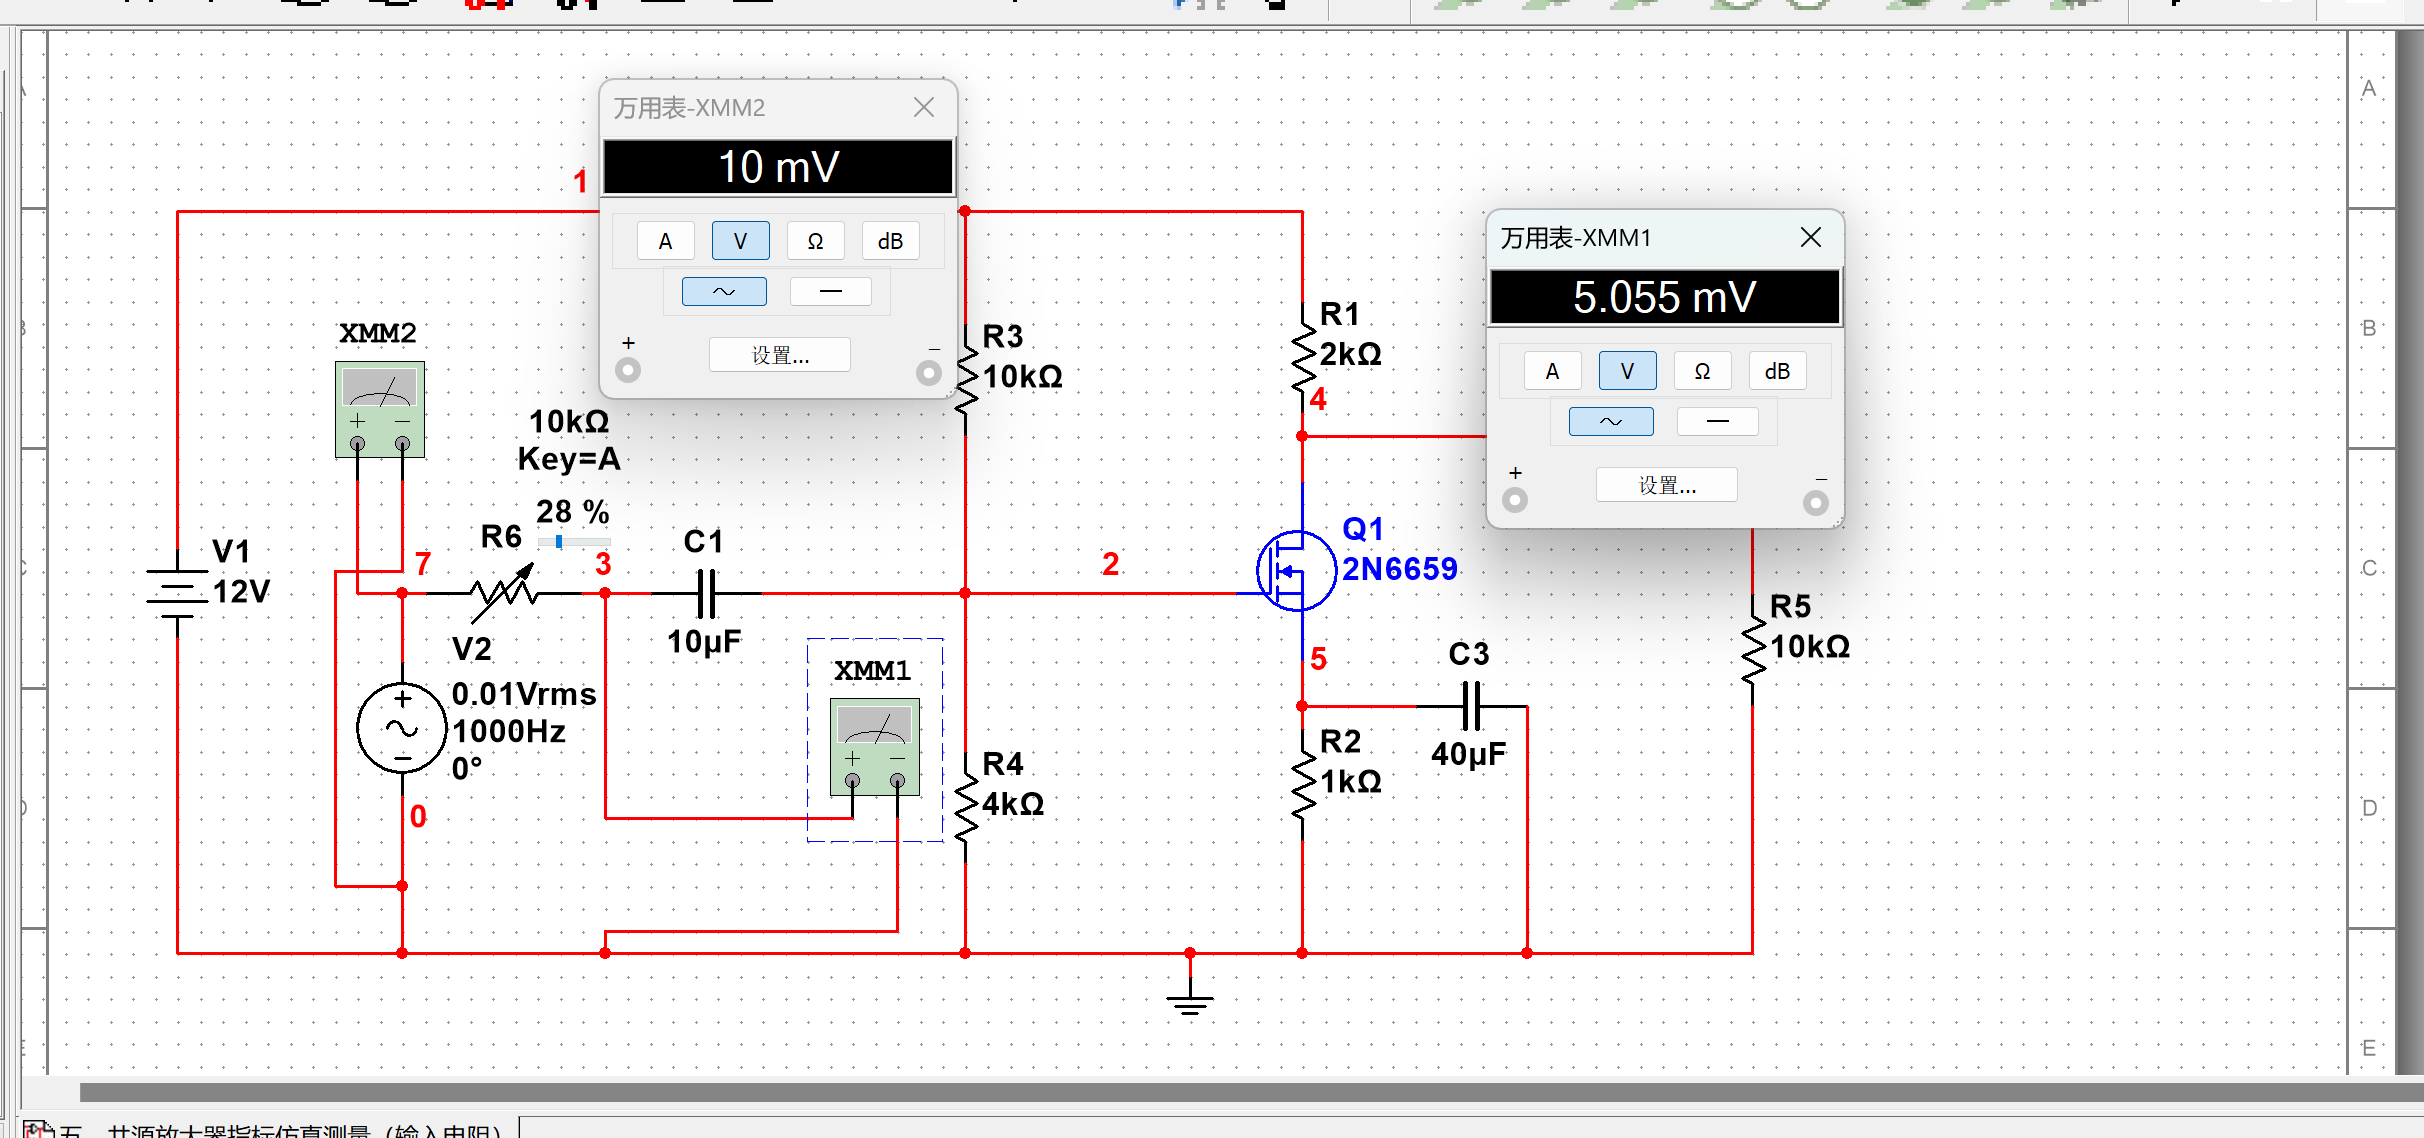
\includegraphics[width=1\linewidth]{4.png}
  \caption{输入电阻测量}
  \label{fig:circuit}
\end{figure}


\subsection{输出电阻测量}
断开负载,测量输出电压$V_{o\ \infty}$,然后串联一个已知电阻$R_{test}$(一般选择$R_L$近似为估算的输出电阻值),保持输入信号不变,重新接入负载测量输出电压,记为$V_{oL}$。
\begin{align*}
  R_{out} &\approx R_1 = 2\ \text{k}\Omega \\
\end{align*}
\begin{itemize}
  \item 选择测试电阻$R_{test} = 2\ \text{k}\Omega$。
  \item 测量得到断开负载时输出电压$V_{o \infty} = 537.126\ \text{mV}$。
  \item 测量得到接入负载输入电压$V_{oL} = 268.613\ \text{mV}$。
\end{itemize}

输出电阻计算公式为:
\[
R_{o} = R_{test} \cdot (\frac{V_{o\ \infty}}{V_{oL}}-1)
\]
代入数据计算得:
\[
R_{in} = 2\ \text{k}\Omega \cdot( \frac{537.126}{268.613}-1)  \approx 2\ \text{k}\Omega
\]
仿真结果与理论计算结果一致。
\FloatBarrier
\begin{figure}[H]
  \centering
  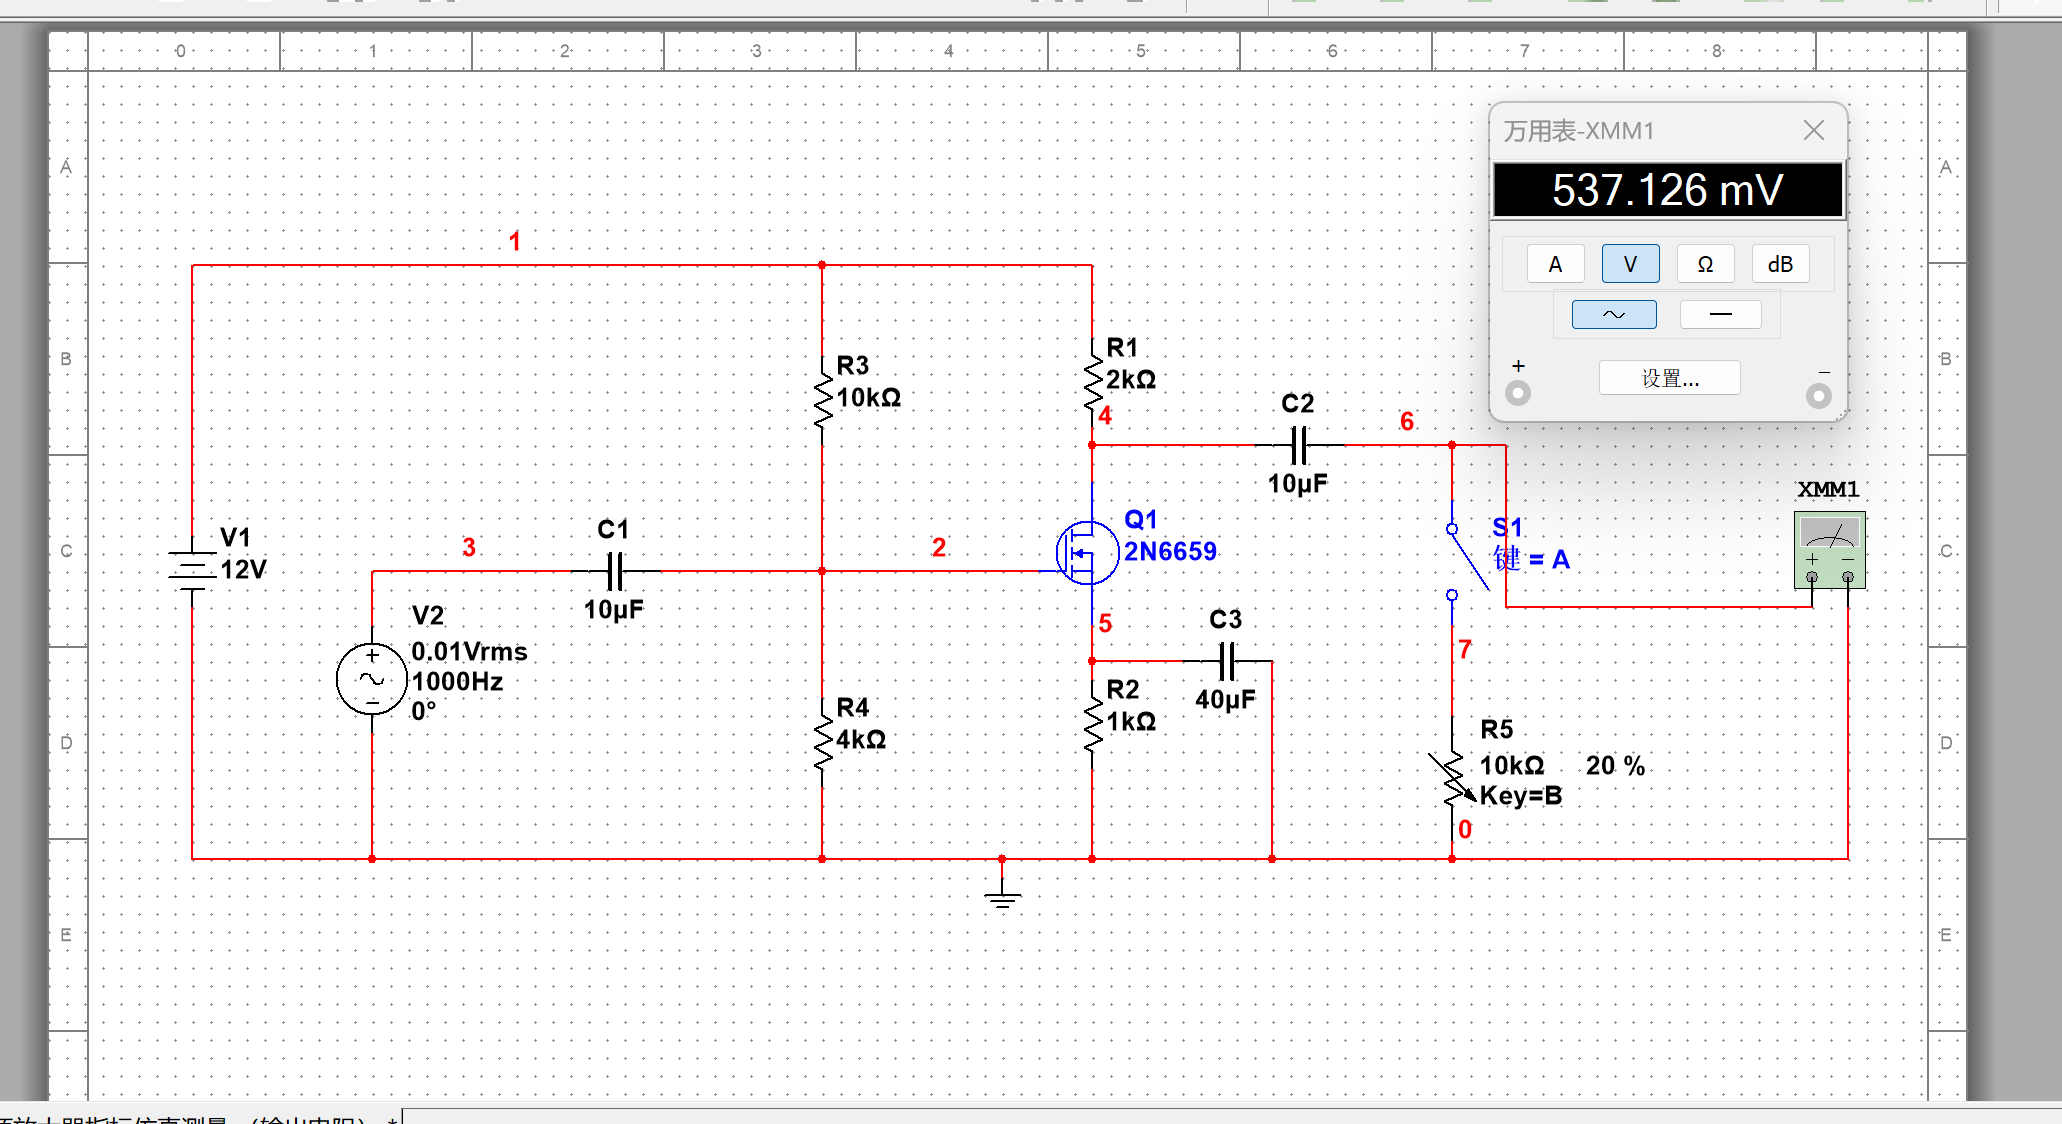
\includegraphics[width=1\linewidth]{5.png}
  \caption{断开负载时输出电压测量}
  \label{fig:circuit}
\end{figure}
\begin{figure}[H]
  \centering
  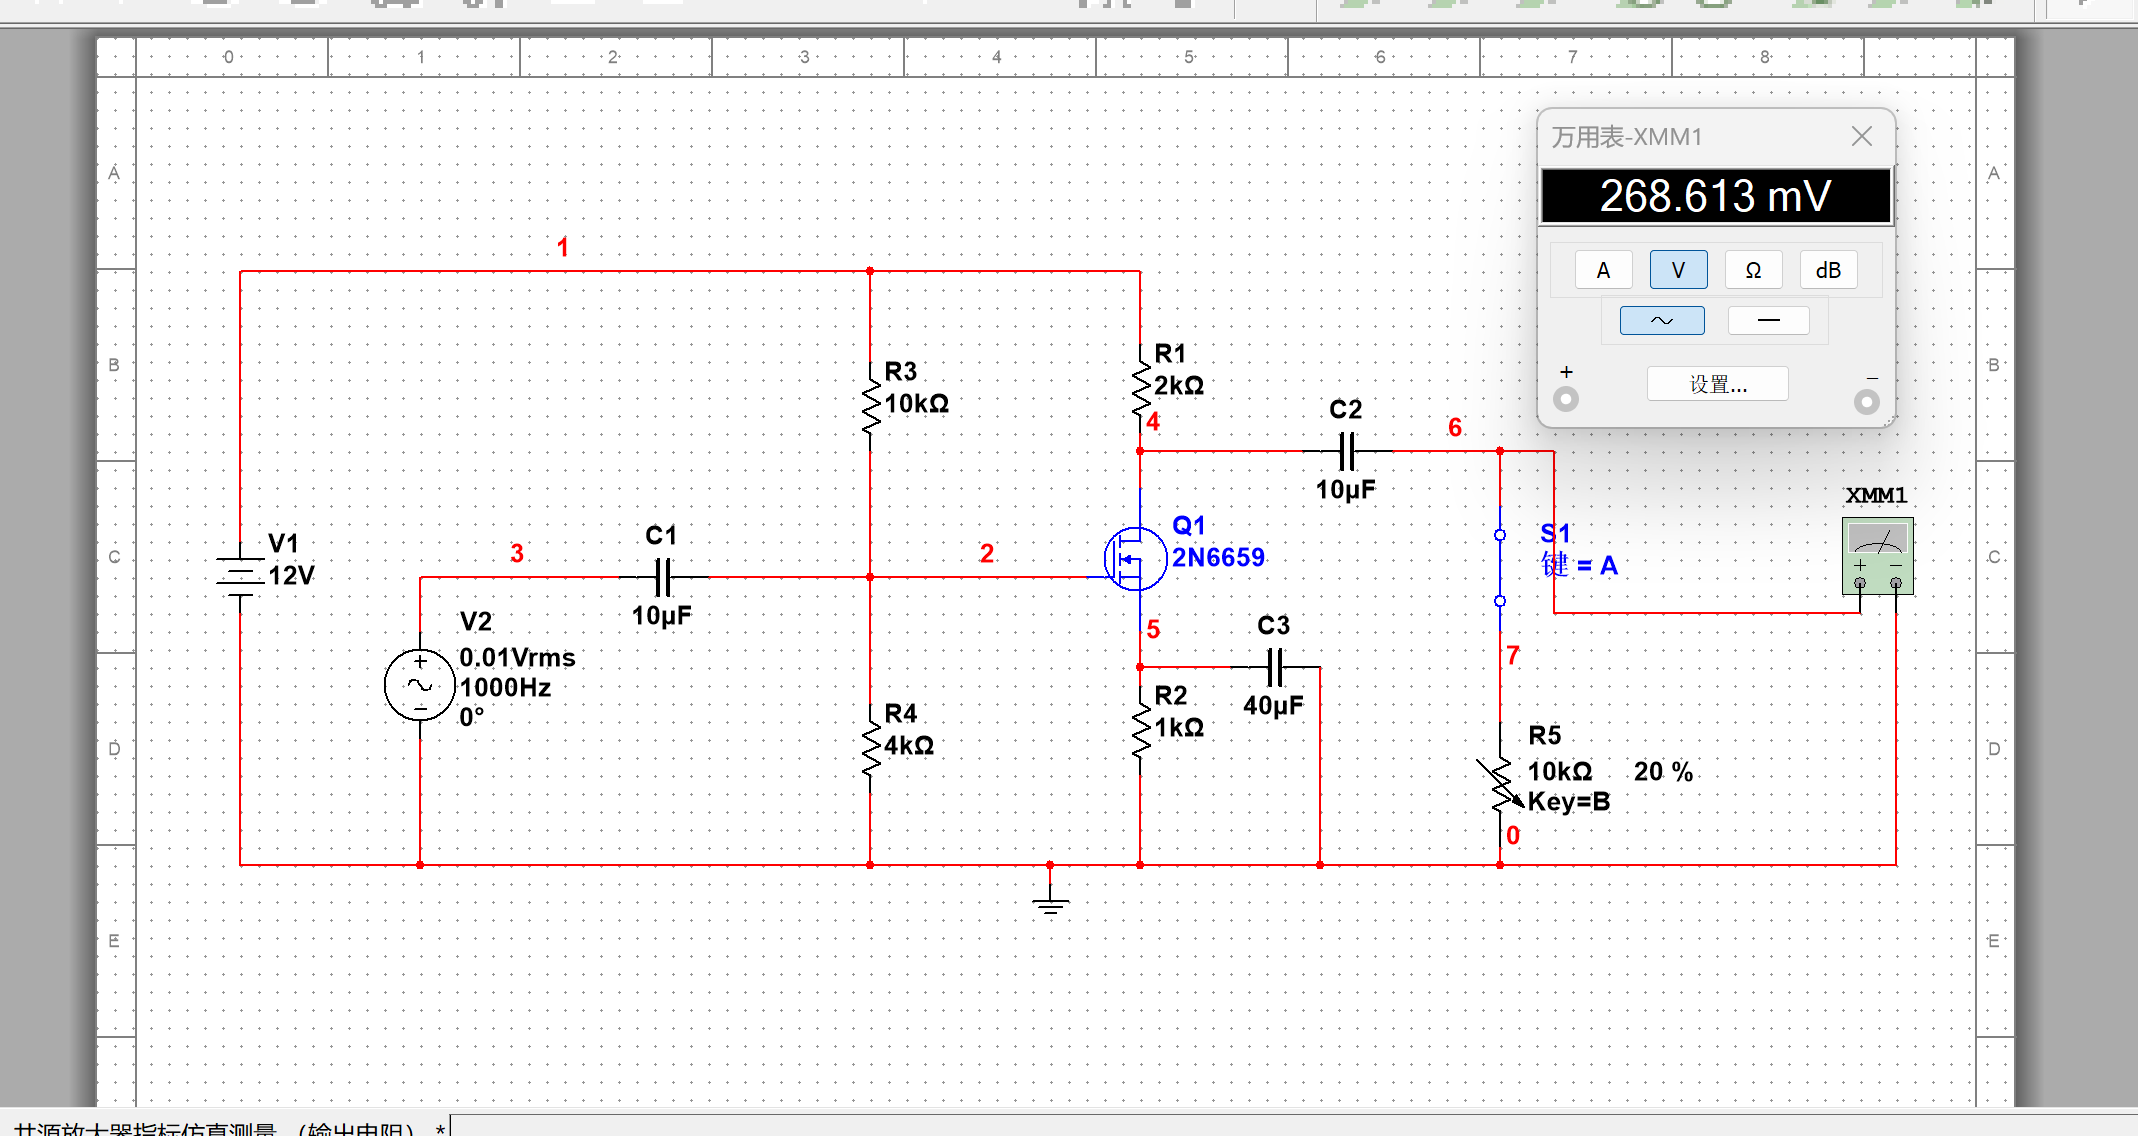
\includegraphics[width=1\linewidth]{6.png}
  \caption{连接负载时输出电压测量}
  \label{fig:circuit}
\end{figure}


\section{心得体会}
通过本次作业,我对共源放大器的工作原理和实际应用有了更深的理解。
实验不仅让我将课堂上学到的理论知识与实践相结合,还让我熟悉了仿真工具的使用,提高了分析电路性能的能力。
在测量直流工作点、增益以及输入输出阻抗的过程中,
我体会到精确的参数选择和细致的操作对结果的准确性至关重要。此外,这次实验让我意识到,在实际电路设计中,
需要综合考虑多个因素进行权衡和优化,这对我未来的学习和工程实践都有很大的启发。

\end{spacing}
\end{document}


 